\documentclass[xcolor=dvipsnames,14pt,professionalfonts]{beamer}
\usepackage{minted}
\usepackage{etoolbox}
\usepackage[T1]{fontenc}
\usepackage{lmodern}
\usepackage[no-math]{fontspec} 
\usetheme{rsmarttraining}
\usefonttheme{professionalfonts}
\usecolortheme{dolphin}

%\definecolor{foreground}{gray}{0}
%\definecolor{background}{gray}{1}
%\definecolor{keyword}{rgb}{0.2,0.2,0.8}
%\definecolor{warning}{rgb}{0.8,0.2,0.2}
%\definecolor{shadow}{gray}{0.35}
%\definecolor{hide}{gray}{0.9}
%\definecolor{figure}{rgb}{1,0.7,0}
%\definecolor{title}{rgb}{25,240,250}
\definecolor{title}{rgb}{0.09,0.30,0.38}
\definecolor{frametitle}{rgb}{1,1,1}
\definecolor{normal}{rgb}{0,0,0}

%\usecolortheme[named=keyword]{structure}

\setbeamercolor{title}{fg=title}
\setbeamercolor{frametitle}{fg=frametitle}
\setbeamercolor{section in toc}{fg=foreground}
\setbeamercolor{normal text}{bg=brown!46,fg=normal}

\setbeamerfont{structure}{family=\fontspec{Georgia},series=\bfseries} 
\setbeamerfont{subtitle}{family=\fontspec{Helvetica},series=\bfseries} 
\begin{document}

\title{KRAD Training}
\subtitle{Maintenance Documents: Part 1}
\author[Leo]{Leo Przybylski}

\usebackgroundtemplate%
{%
    
\includegraphics[width=\paperwidth,height=\paperheight]{../img/header.png}%
}

{
\usebackgroundtemplate{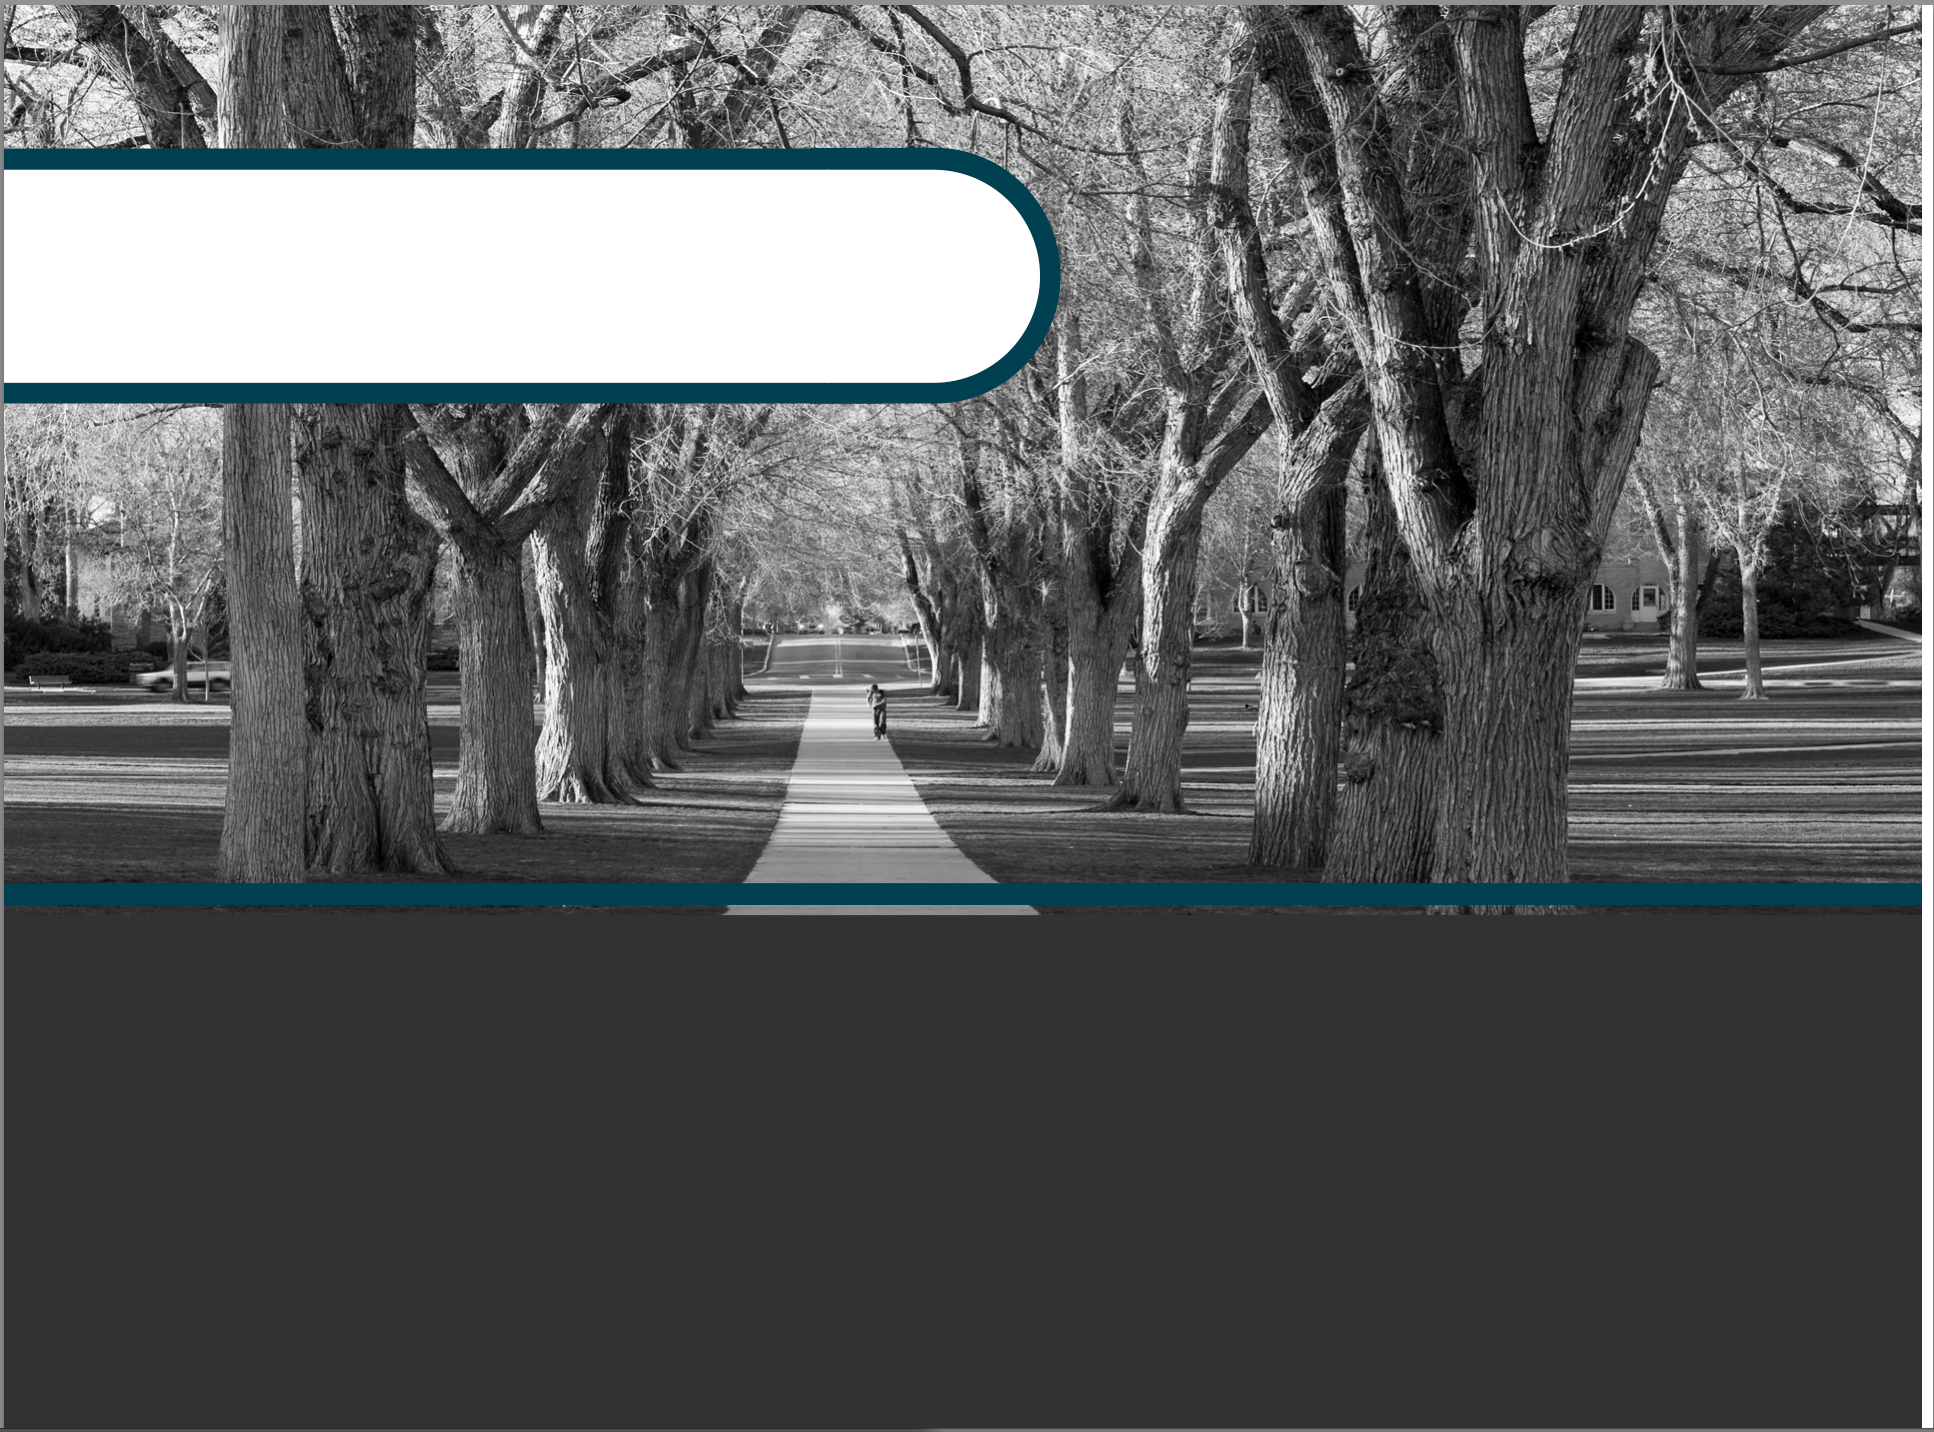
\includegraphics[width=\paperwidth]{../img/title.png}}%
\begin{frame}[plain]
  \titlepage
\end{frame}
}

\begin{frame}{Overview}
  \begin{itemize}
  \item Maintenance Documents and Transactional Documents
  \item Differences between KRAD and KNS
  \item Uif-MaintenanceView
  \item Uif-MaintenanceGridSection
  \end{itemize}
\end{frame}

\begin{frame}{Maintenance and Transactional Documents}
  \begin{itemize}
    \item Generally speaking, Documents are carriages for business
      objects through workflow (which is really just a routing system
      more than BPM engine as the name suggests).
    \item Maintenance Documents are tightly coupled to modify a given
      business object externally.
    \item Transactional Documents are themselves the business object
      and can be used as a more possible alternative.
  \end{itemize}
\end{frame}

\begin{frame}{Differences between KRAD and KNS}
  \begin{itemize}
  \item KNS Maintenance Documents had a static view where the
    developer had next to no control over.
  \item KRAD Maintenance Documents are minor bean instances that
    essentially metadata for something called a
    \texttt{Uif-MaintenanceView}. Since Views are exposed in KRAD
    through the DataDictionary, this is the opposite situation as what
    exists in the KNS. Now the developer has complete control over the
    view of a Maintenance Document.
  \end{itemize}
\end{frame}

\begin{frame}{Differences between KRAD and KNS}
  \begin{itemize}
  \item In KRAD, now there are 3 bean definitions that require knowing
    what the \texttt{dataObjectClass} is: DataObjectEntry,
    uifMaintenanceDocumentEntry, and the Uif-MaintenanceView.
  \item in KNS, the MaintenanceDocumentEntry had special beans that
    needed to be used.
  \item in KRAD, since Uif-MaintenanceView is just a view, and
    elements from the UIF can be added the the Uif-MaintenanceView.
  \end{itemize}
\end{frame}

\begin{frame}[fragile]{Uif-MaintenanceView}
  \begin{itemize}
    \item View intended for maintenance documents
    \item Includes items for workflow actions (buttons along the
      bottom), and the Document Overview
    \item When adding items, be sure to use:
      \begin{minted}[fontsize=\scriptsize]{xml}
<list merge=''true''> ... </list>
      \end{minted}
    \item Requires \texttt{dataObjectClassName} to be set. This will
      bind the form attached to the view to the
      \texttt{uifMaintenanceDocumentEntry} instance mapped to the same \texttt{dataObjectClass}
      
    \end{itemize}
\end{frame}

\begin{frame}{Uif-MaintenanceGridSection}
  \begin{itemize}
  \item Special Grid section that uses the
    \texttt{oldMaintainableObject} if there is one. This is what makes
    it possible to show changes side-by-side
  \item It's possible to create a maintenance document without this,
    but you lose the ability to see what fields changed.
    \end{itemize}
\end{frame}

\end{document}
